%%%%%%%%%%%%%%%%%%%%%%%%%%%%%%%%%%%%%%%%%%%%%%%%%%%%%%%%%%%%%%%%%%%%%%%%%%%%%%%
%% 2.- DESARROLLO DEL PROYECTO
%%%%%%%%%%%%%%%%%%%%%%%%%%%%%%%%%%%%%%%%%%%%%%%%%%%%%%%%%%%%%%%%%%%%%%%%%%%%%%%

\cleardoublepage
\chapter{Desarrollo del proyecto}
\chaptermark{Desarrollo del proyecto}

\label{chap:desarrolloProyecto} % etiqueta para poder referenciar luego en el texto con ~\ref{sec:intro}
% \addcontentsline{toc}{chapter}{Introducción, Objetivos, Metodología y Planificación

En las siguientes secciones se detalla de forma estructurada el desarrollo de cada una de las partes que componen este proyecto.


\section{Programación iPro}
\label{sec:programacionipro}
Como ya se ha explicado en los capítulos anteriores, el destino del iPro es la programación de la UTA existente en el supermercado. En el \hyperref[chap:anexoUTA]{Anexo~\ref{chap:anexoUTA}} se describe detalladamente qué es una UTA y todos los elementos de los que se puede componer. Para el caso que nos atañe, la \hyperref[tab:especificacionesUTA]{Tabla~\ref{tab:especificacionesUTA}} recoge las especificaciones concretas del control.

\begin{table}[H]
    %\centering
    \begin{center}
      \setlength\arrayrulewidth{2pt}
      \resizebox{0.8\linewidth}{!}{\begin{tabular}{ | c | c c c c | }
        %\Cline{2pt}{2-5}
        \hhline{|*{5}{-}}
        \cellcolor{lightgray}\textbf{GRUPO} & \multicolumn{1}{c|}{\cellcolor{lightgray}\textbf{Entrada analógica}} & \multicolumn{1}{c|}{\cellcolor{lightgray}\textbf{Salida analógica}} & \multicolumn{1}{c|}{\cellcolor{lightgray}\textbf{Entrada digital}} & \cellcolor{lightgray}\textbf{Salida digital}   \\ \hline
        \footnotesize{\textbf{Ventiladores}} &  & \parbox[c][1.6cm]{0.2\linewidth}{\centering\footnotesize{Ventilador impulsión\\Ventilador retorno}}  & \parbox[c][2.6cm]{0.2\linewidth}{\centering\footnotesize{Seguridad Ventilador impulsión\\Seguridad Ventilador retorno}} &  \\ \hline
        \footnotesize{\textbf{Filtros}} & & & \footnotesize{\parbox[c][2cm]{0.2\linewidth}{\centering{Filtro entrada\\Filtro salida\\Filtro retorno}}} & \\ \hline
        \footnotesize{\textbf{Humectador}} & \footnotesize{\parbox[c][1.2cm]{0.2\linewidth}{\centering{Humedad de retorno\\Humedad exterior}}} & & \centering\footnotesize{Indicador nivel agua} & \footnotesize{ON/OFF Humectador} \\ \hline
        \footnotesize{\textbf{Intercambiador de calor}} & \footnotesize{\parbox[c][1.2cm]{0.2\linewidth}{\centering{Temp. impulsión agua\\Temp. retorno agua}}} & & & \footnotesize{Válvula de agua}\\ \hline
        \footnotesize{\textbf{E/S de aire}} & \footnotesize{\parbox[c][2.7cm]{0.2\linewidth}{\centering{Temp. impulsión aire\\Temp. retorno aire\\Temp. extracción aire\\Temp. aire exterior}}} & & & \\ \hline

      \end{tabular}}
      \caption{Especificaciones E/S UTA.}
      \label{tab:especificacionesUTA}
    \end{center}
  \end{table}

Las especificaciones de funcionamiento son las siguientes:

\begin{itemize}
  \item \textbf{Compuertas:} No existen compuertas regulables.
  \item \textbf{Filtros:} La señal digital de los filtros indica si están sucios o no. Existen tres filtros: de entrada de aire, de retorno de aire y de impulsión de aire.
  \item \textbf{Ventiladores:} 
  \begin{itemize}
    \item La velocidad de los ventiladores se regula mediante una señal 0-10V. Existen dos ventiladores, uno para la entrada y otro para la salida de aire. La velocidad de ambos debe estar coordinada y ser la misma en cada momento.
    \item La señal digital en los ventiladores indica fallo en los mismos.
    \item La velocidad debe ser ajustable de forma automática o de forma manual:
    \begin{itemize}
      \item La regulación automática ajusta la velocidad del ventilador en función de la diferencia de temperatura con la consigna.
      \item La regulación manual de la velocidad se establece en tres rangos parametrizables: alta, media y baja.
    \end{itemize}
  \end{itemize} 
  \item \textbf{Humectador:} 
  \begin{itemize}
    \item Se establece una consigna de humedad.
    \item A partir de las mediciones de humedad del aire que entra y sale se activa la humectación o no.
    \item El indicador de nivel del humectador indica si éste está lleno o no.
  \end{itemize}
  \item \textbf{Intercambiador de calor:}
  \begin{itemize}
    \item Debe existir un aviso que indique si el fluido está a una temperatura acorde para alcanzar la consigna deseada.
    \item Mientras la UTA esté en funcionamiento, la válvula que lleva el fluido hasta el intercambiador debe estar abierta.
  \end{itemize}
  \item \textbf{E/S de aire:}
  \begin{itemize}
    \item La temperatura de retorno es la usada como referencia para el control de temperatura del aire.
    \item El control de temperatura se establece según el modo de funcionamiento: verano (frío) o invierno (calor).
    \item Las curva de funcionamiento para cada uno de los modos es la de la \hyperref[figura:curvasModos]{Figura~\ref{figura:curvasModos}}:
  \end{itemize}
\end{itemize}

\begin{figure}[H]
  \centering
  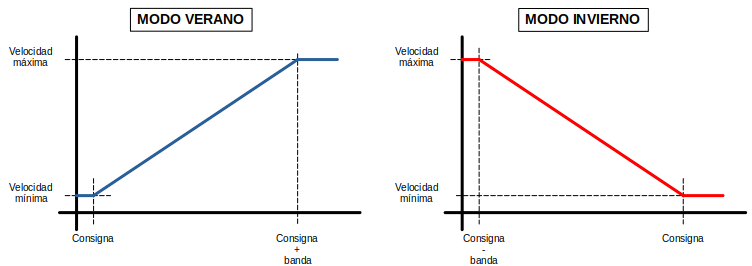
\includegraphics[width=\textwidth, keepaspectratio]{img/curvaModos}
  \caption{Modos de funcionamiento}
  \label{figura:curvasModos}
\end{figure}



El \hyperref[chap:anexoProgramaUTA]{Anexo~\ref{chap:anexoProgramaUTA}} presenta la lógica de funcionamiento del programa de la UTA. Los parámetros necesarios para la configuración del controlador son los de la \hyperref[tab:parametrosUTA]{Tabla~\ref{tab:parametrosUTA}}.

\begin{center}
  \begin{longtable}{|p{3cm}|p{3cm}|p{9cm}|}
  \caption{Parámetros de configuración de la UTA.} \label{tab:parametrosUTA} \\
  
  \hline \cellcolor{lightgray}\centering\textbf{GRUPO} & \cellcolor{lightgray}\centering\textbf{PARÁMETRO} & \cellcolor{lightgray}\textbf{DESCRIPCIÓN} \\ \hline 
  \endfirsthead
  
  \multicolumn{3}{c}%
  {\footnotesize{\bfseries \tablename\ \thetable{} ...continuación de la página anterior.}} \\
  \hline \cellcolor{lightgray}\textbf{GRUPO} & \cellcolor{lightgray}\textbf{PARÁMETRO} & \cellcolor{lightgray}\textbf{DESCRIPCIÓN} \\ \hline 
  \endhead
  
  \hline  \multicolumn{3}{c}%
  {\footnotesize{\bfseries \tablename\ \thetable{} continua en la página siguiente...}} \\
  \endfoot
  
  \hline
  \endlastfoot
  
      \multirow{6}{*}\centering{Configuración Equipo} & \centering\textbf{CNF01} & Habilitar módulos de expansión (DIN4/DIN10) \\ \cline{2-3}
      & \centering\textbf{HUM01} & Establecer consigna de humedad en \%HR \\ \cline{2-3}
      & \centering\textbf{HUM02} & Establecer banda para control de humedad, en \%HR \\ \cline{2-3}
      & \centering\textbf{TMP01} & Establecer consigna de temperatura en $^{\circ}$C \\ \cline{2-3}
      & \centering\textbf{TMP02} & Establecer banda de temperatura para la
      regulación en el modo invierno ($^{\circ}$C) \\ \cline{2-3}
      & \centering\textbf{TMP03} & Establecer banda de temperatura para la
      regulación en el modo verano ($^{\circ}$C) \\ \hline
      \multirow{12}{*}{\centering{Ventiladores}} & \centering\textbf{FAN01} & Establecer valor de velocidad baja \\ \cline{2-3}
      & \centering\textbf{FAN02} & Establecer valor de velocidad media \\ \cline{2-3}
      & \centering\textbf{FAN03} & Establecer valor de velocidad alta \\ \cline{2-3}
      & \centering\textbf{FAN04} & Establecer valor de velocidad mínima para la
      regulación automática \\ \cline{2-3}
      & \centering\textbf{FAN05} & Establecer valor de velocidad máxima para la
      regulación automática \\ \cline{2-3}
      & \centering\textbf{FAN06} & Establecer banda de velocidad para la regulación
      automática \\ \cline{2-3}
      & \centering\textbf{FAN07} & Tiempo de retardo de activación de alarma en
      ventilador de impulsión, en segundos \\ \cline{2-3}
      & \centering\textbf{FAN08} & Tiempo de retardo de desactivación de alarma en
      ventilador de impulsión, en segundos \\ \cline{2-3}
      & \centering\textbf{FAN09} & Número de alarmas en el ventilador de impulsión
      hasta bloqueo \\ \cline{2-3}
      & \centering\textbf{FAN10} & Tiempo de retardo de activación de alarma en
      ventilador de retorno, en segundos \\ \cline{2-3}
      & \centering\textbf{FAN11} & Tiempo de retardo de desactivación de alarma en
      ventilador de retorno, en segundos \\ \cline{2-3}
      & \centering\textbf{FAN12} & Número de alarmas en el ventilador de retorno
      hasta bloqueo \\ \hline
      \multirow{6}{*}{\centering{Filtros}} & \centering\textbf{FIL01} & Retardo de activación de aviso en filtro de entrada
      de aire en segundos \\ \cline{2-3}
      & \centering\textbf{FIL02} & Retardo de desactivación de aviso en filtro de
      entrada de aire en segundos \\ \cline{2-3}
      & \centering\textbf{FIL03} & Retardo de activación de aviso en filtro de
      impulsión de aire en segundos \\ \cline{2-3}
      & \centering\textbf{FIL04} & Retardo de desactivación de aviso en filtro de
      impulsión de aire en segundos \\ \cline{2-3}
      & \centering\textbf{FIL05} & Retardo de activación de aviso en filtro de retorno
      de aire en segundos \\ \cline{2-3}
      & \centering\textbf{FIL06} & Retardo de desactivación de aviso en filtro de
      retorno de aire en segundos \\ \hline
      \multirow{43}{*}\centering{Entradas digitales} & \centering\textbf{DIG01} & \footnotesize{\textbf{INV(FALSE)/DIR(TRUE)}: polaridad inversa o directa} \\ \cline{2-2}
      & \centering\textbf{DIG02} & \footnotesize{\textbf{0=No utilizado}: entrada sin función asociada} \\ \cline{2-2}
      & \centering\textbf{DIG03} & \footnotesize{\textbf{1=ON-OFF}: Interruptor de ON/OFF remoto} \\ \cline{2-2}
      & \centering\textbf{DIG04} & \footnotesize{\textbf{2=DI. Ventilador Impulsión}: seguridad ventilador impulsión} \\ \cline{2-2}
      & \centering\textbf{DIG05} & \footnotesize{\textbf{3=DI. Ventilador retorno}: seguridad ventilador retorno} \\ \cline{2-2}
      & \centering\textbf{DIG06} & \footnotesize{\textbf{4=DI. Nivel Humectador}: seguridad nivel humectador} \\ \cline{2-2}
      & \centering\textbf{DIG07} & \footnotesize{\textbf{5=DI. Filtro entrada aire}: seguridad filtro entrada aire} \\ \cline{2-2}
      & \centering\textbf{DIG08} & \footnotesize{\textbf{6=DI. Filtro impulsión aire}: seguridad filtro impulsión aire} \\ \cline{2-2}
      & \centering\textbf{DIG09} & \footnotesize{\textbf{7=DI. Filtro retorno aire}: seguridad filtro retorno aire} \\ \cline{2-2}
      & \centering\textbf{DIG10} &  \\ \cline{2-2}
      & \centering\textbf{DIG11} &  \\ \cline{2-2}
      & \centering\textbf{DIG12} &  \\ \cline{2-2}
      & \centering\textbf{DIG13} &  \\ \cline{2-2}
      & \centering\textbf{DIG14} &  \\ \cline{2-2}
      & \centering\textbf{DIG15} &  \\ \cline{2-2}
      & \centering\textbf{DIG16} &  \\ \cline{2-2}
      & \centering\textbf{DIG17} &  \\ \cline{2-2}
      & \centering\textbf{DIG18} &  \\ \cline{2-2}
      & \centering\textbf{DIG19} &  \\ \cline{2-2}
      & \centering\textbf{DIG20} &  \\ \cline{2-2}
      & \centering\textbf{DIG21} &  \\ \cline{2-2}
      & \centering\textbf{DIG22} &  \\ \cline{2-2}
      & \centering\textbf{DIG23} &  \\ \cline{2-2}
      & \centering\textbf{DIG24} &  \\ \cline{2-2}
      & \centering\textbf{DIG25} &  \\ \cline{2-2}
      & \centering\textbf{DIG26} &  \\ \cline{2-2}
      & \centering\textbf{DIG27} &  \\ \cline{2-2}
      & \centering\textbf{DIG28} &  \\ \cline{2-2}
      & \centering\textbf{DIG29} &  \\ \cline{2-2}
      & \centering\textbf{DIG30} &  \\ \cline{2-2}
      & \centering\textbf{DIG31} &  \\ \cline{2-2}
      & \centering\textbf{DIG32} &  \\ \cline{2-2}
      & \centering\textbf{DIG33} &  \\ \cline{2-2}
      & \centering\textbf{DIG34} &  \\ \cline{2-2}
      & \centering\textbf{DIG35} &  \\ \cline{2-2}
      & \centering\textbf{DIG36} &  \\ \cline{2-2}
      & \centering\textbf{DIG37} &  \\ \cline{2-2}
      & \centering\textbf{DIG38} &  \\ \cline{2-2}
      & \centering\textbf{DIG39} &  \\ \cline{2-2}
      & \centering\textbf{DIG40} &  \\ \cline{2-2}
      & \centering\textbf{DIG41} &  \\ \cline{2-2}
      & \centering\textbf{DIG42} &  \\ \cline{2-2}
      & \centering\textbf{DIG43} &  \\ \hline
      \multirow{43}{*}\centering\small{Sondas analógicas} & \centering\textbf{PBS01} & \footnotesize{\textbf{0=no usado}: sonda sin función} \\ \cline{2-2}
      & \centering\textbf{PBS02} & \footnotesize{\textbf{1=Ta impulsión aire}} \\ \cline{2-2}
      & \centering\textbf{PBS03} & \footnotesize{\textbf{2=Ta retorno aire}} \\ \cline{2-2}
      & \centering\textbf{PBS04} & \footnotesize{\textbf{3=Ta impulsión agua}} \\ \cline{2-2}
      & \centering\textbf{PBS05} & \footnotesize{\textbf{4=Ta retorno agua}} \\ \cline{2-2}
      & \centering\textbf{PBS06} & \footnotesize{\textbf{5=Ta extracción aire}} \\ \cline{2-2}
      & \centering\textbf{PBS07} & \footnotesize{\textbf{6=Ta aire extraído}} \\ \cline{2-2}
      & \centering\textbf{PBS08} & \footnotesize{\textbf{7=Ta extracción aire}} \\ \cline{2-2}
      & \centering\textbf{PBS09} & \footnotesize{\textbf{8=Humedad de retorno}} \\ \cline{2-2}
      & \centering\textbf{PBS10} & \footnotesize{\textbf{9=Humedad exterior}} \\ \cline{2-2}
      & \centering\textbf{PBS11} &  \\ \cline{2-2}
      & \centering\textbf{PBS12} &  \\ \cline{2-2}
      & \centering\textbf{PBS13} &  \\ \cline{2-2}
      & \centering\textbf{PBS14} &  \\ \cline{2-2}
      & \centering\textbf{PBS15} &  \\ \cline{2-2}
      & \centering\textbf{PBS16} &  \\ \cline{2-2}
      & \centering\textbf{PBS17} &  \\ \cline{2-2}
      & \centering\textbf{PBS18} &  \\ \cline{2-2}
      & \centering\textbf{PBS19} &  \\ \cline{2-2}
      & \centering\textbf{PBS20} &  \\ \cline{2-2}
      & \centering\textbf{PBS21} &  \\ \cline{2-2}
      & \centering\textbf{PBS22} &  \\ \cline{2-2}
      & \centering\textbf{PBS23} &  \\ \cline{2-2}
      & \centering\textbf{PBS24} &  \\ \cline{2-2}
      & \centering\textbf{PBS25} &  \\ \cline{2-2}
      & \centering\textbf{PBS26} &  \\ \cline{2-2}
      & \centering\textbf{PBS27} &  \\ \hline
      \multirow{43}{*}\centering{Rele salida} & \centering\textbf{RLO01} & \footnotesize{\textbf{0=No usado}:relé sin función asociada} \\ \cline{2-2}
      & \centering\textbf{RLO02} & \footnotesize{\textbf{1=Válvula de 3 vías}: activación válvula de agua} \\ \cline{2-2}
      & \centering\textbf{RLO03} & \footnotesize{\textbf{2=Humectador}: activación humectador} \\ \cline{2-2}
      & \centering\textbf{RLO04} & \footnotesize{\textbf{3=Alarma}: activación alarma} \\ \cline{2-2}
      & \centering\textbf{RLO05} &  \\ \cline{2-2}
      & \centering\textbf{RLO06} &  \\ \cline{2-2}
      & \centering\textbf{RLO07} &  \\ \cline{2-2}
      & \centering\textbf{RLO08} &  \\ \cline{2-2}
      & \centering\textbf{RLO09} &  \\ \cline{2-2}
      & \centering\textbf{RLO10} &  \\ \cline{2-2}
      & \centering\textbf{RLO11} &  \\ \cline{2-2}
      & \centering\textbf{RLO12} &  \\ \cline{2-2}
      & \centering\textbf{RLO13} &  \\ \cline{2-2}
      & \centering\textbf{RLO14} &  \\ \cline{2-2}
      & \centering\textbf{RLO15} &  \\ \cline{2-2}
      & \centering\textbf{RLO16} &  \\ \cline{2-2}
      & \centering\textbf{RLO17} &  \\ \cline{2-2}
      & \centering\textbf{RLO18} &  \\ \cline{2-2}
      & \centering\textbf{RLO19} &  \\ \cline{2-2}
      & \centering\textbf{RLO20} &  \\ \cline{2-2}
      & \centering\textbf{RLO21} &  \\ \cline{2-2}
      & \centering\textbf{RLO22} &  \\ \cline{2-2}
      & \centering\textbf{RLO23} &  \\ \cline{2-2}
      & \centering\textbf{RLO24} &  \\ \cline{2-2}
      & \centering\textbf{RLO25} &  \\ \cline{2-2}
      & \centering\textbf{RLO26} &  \\ \cline{2-2}
      & \centering\textbf{RLO27} &  \\ \cline{2-2}
      & \centering\textbf{RLO28} &  \\ \cline{2-2}
      & \centering\textbf{RLO29} &  \\ \cline{2-2}
      & \centering\textbf{RLO30} &  \\ \cline{2-2}
      & \centering\textbf{RLO31} &  \\ \cline{2-2}
      & \centering\textbf{RLO32} &  \\ \cline{2-2}
      & \centering\textbf{RLO33} &  \\ \cline{2-2}
      & \centering\textbf{RLO34} &  \\ \cline{2-2}
      & \centering\textbf{RLO35} &  \\ \cline{2-2}
      & \centering\textbf{RLO36} &  \\ \hline
      \multirow{43}{*}\centering{Salidas} & \centering\textbf{ANA01} & \footnotesize{\textbf{0=No utilizado}: salida sin función asociada} \\ \cline{2-2}
      analógicas & \centering\textbf{ANA02} & \footnotesize{\textbf{1=Vel. Ventilador imp.}: salida analógica para regular la} \\ \cline{2-2}
      & \centering\textbf{ANA03} & \footnotesize{velocidad del ventilador de impulsión de aire} \\ \cline{2-2}
      & \centering\textbf{ANA04} & \footnotesize{\textbf{2=Vel. Ventilador ret.}: salida analógica para regular la} \\ \cline{2-2}
      & \centering\textbf{ANA05} & \footnotesize{velocidad del ventilador de retorno de aire} \\ \cline{2-2}
      & \centering\textbf{ANA06} &  \\ \cline{2-2}
      & \centering\textbf{ANA07} &  \\ \cline{2-2}
      & \centering\textbf{ANA08} &  \\ \cline{2-2}
      & \centering\textbf{ANA09} &  \\ \cline{2-2}
      & \centering\textbf{ANA10} &  \\ \cline{2-2}
      & \centering\textbf{ANA11} &  \\ \cline{2-2}
      & \centering\textbf{ANA12} &  \\ \cline{2-2}
      & \centering\textbf{ANA13} &  \\ \cline{2-2}
      & \centering\textbf{ANA14} &  \\ \cline{2-2}
      & \centering\textbf{ANA15} &  \\ 
  \end{longtable}
  \end{center}

\section{Diseño Pantalla para el control}
\label{sec:programacionpantalla}
Desde el programa Visoprog, donde se diseña la pantalla, se importan las variables del programa creado con el software ISaGRAF. Para ello, Visoprog tiene dos opciones de importación: directamente desde un proyecto ISaGRAF o desde una hoja excel o fichero csv. 

El diseño realizado se compone de las ventanas de la \hyperref[figura:ventanas]{Figura~\ref{figura:ventanas}}, su funcionamiento se describe en el manual del \hyperref[chap:anexoManualUTA]{Anexo~\ref{chap:anexoManualUTA}}:

\begin{figure}[H]
  \centering
   \subfigure[Logo de inicio]{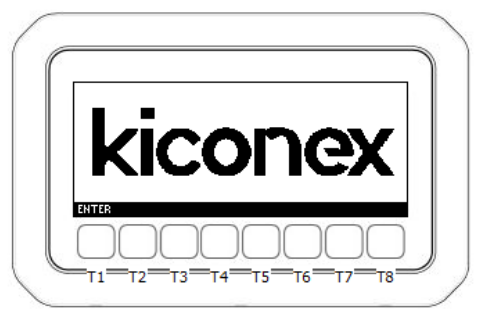
\includegraphics[width=0.4\textwidth]{img/vent0}}
   \subfigure[Pantalla principal]{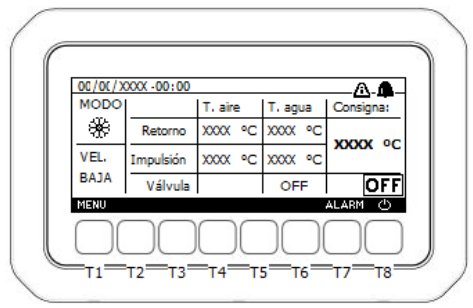
\includegraphics[width=0.4\textwidth]{img/vent1}}
 \end{figure}

 \begin{figure}[H]
  \centering
   \subfigure[Menú]{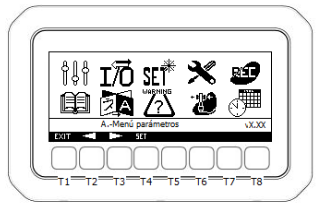
\includegraphics[width=0.4\textwidth]{img/vent2}}
   \subfigure[Menú de parámetros]{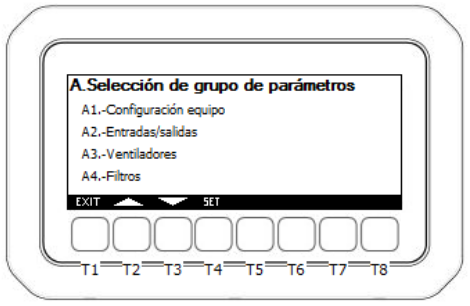
\includegraphics[width=0.4\textwidth]{img/vent3}}
 \end{figure}

 \begin{figure}[H]
  \centering
   \subfigure[Configuración de sondas analógicas]{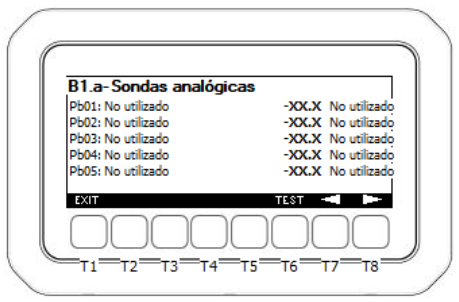
\includegraphics[width=0.4\textwidth]{img/vent4}}
   \subfigure[Configuración de entradas digitales]{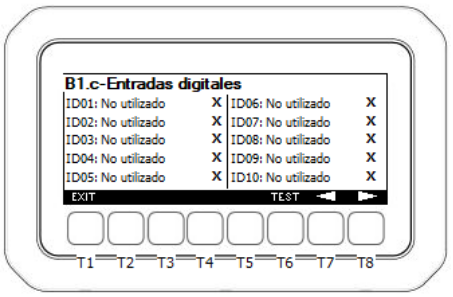
\includegraphics[width=0.4\textwidth]{img/vent5}}
 \end{figure}

 \begin{figure}[H]
  \centering
   \subfigure[Configuración de relés de salida]{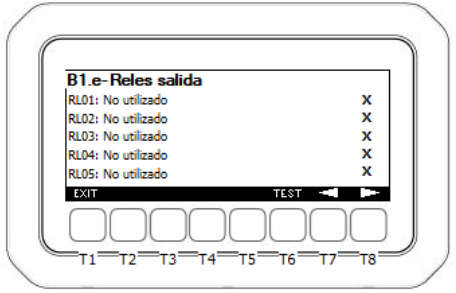
\includegraphics[width=0.4\textwidth]{img/vent6}}
   \subfigure[Configuración de sondas analógicas]{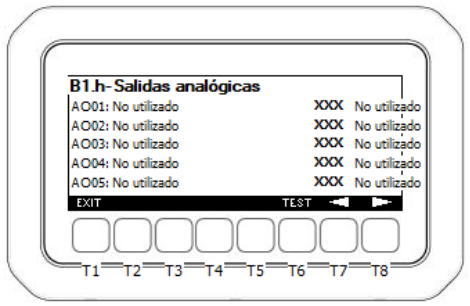
\includegraphics[width=0.4\textwidth]{img/vent7}}
 \end{figure}

 \begin{figure}[H]
  \centering
   \subfigure[Consigna de humedad]{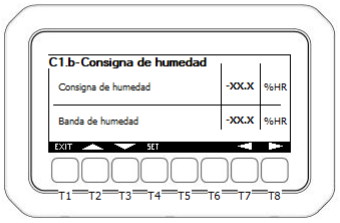
\includegraphics[width=0.4\textwidth]{img/vent8}}
   \subfigure[Menú de servicio]{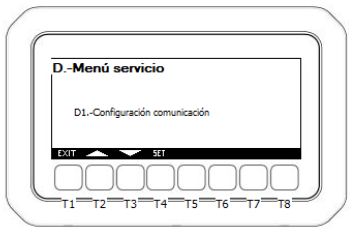
\includegraphics[width=0.4\textwidth]{img/vent9}}
 \end{figure}

 \begin{figure}[H]
  \centering
   \subfigure[Configuración de comunicación]{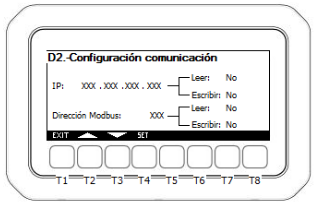
\includegraphics[width=0.4\textwidth]{img/vent10}}
   \subfigure[Registro de alarmas]{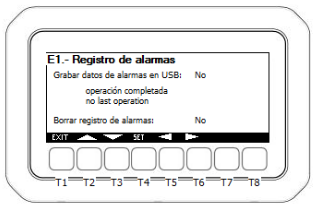
\includegraphics[width=0.4\textwidth]{img/vent11}}
 \end{figure}

 \begin{figure}[H]
  \centering
   \subfigure[Registro de datos]{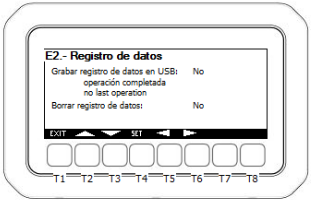
\includegraphics[width=0.4\textwidth]{img/vent12}}
   \subfigure[Habilitar el registro de datos]{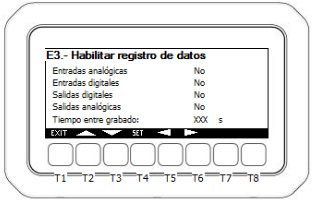
\includegraphics[width=0.4\textwidth]{img/vent13}}
 \end{figure}

 \begin{figure}[H]
  \centering
   \subfigure[Menú de carga/descarga de parámetros]{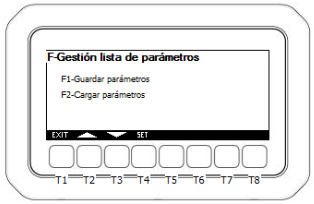
\includegraphics[width=0.4\textwidth]{img/vent14}}
   \subfigure[Guardar parámetros]{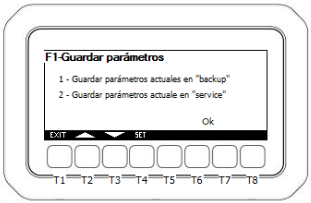
\includegraphics[width=0.4\textwidth]{img/vent15}}
 \end{figure}

 \begin{figure}[H]
  \centering
   \subfigure[Cargar parámetros]{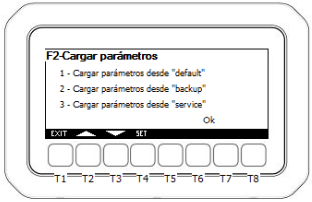
\includegraphics[width=0.4\textwidth]{img/vent16}}
   \subfigure[Cambio de idioma]{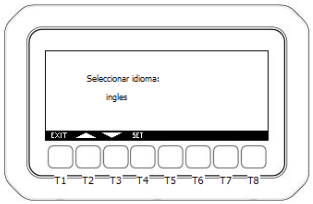
\includegraphics[width=0.4\textwidth]{img/vent17}}
 \end{figure}

 \begin{figure}[H]
  \centering
   \subfigure[Visualización de avisos]{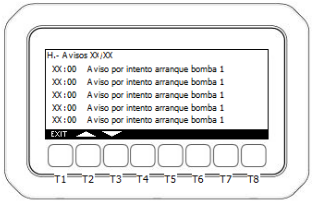
\includegraphics[width=0.4\textwidth]{img/vent18}}
   \caption{Diseño de las ventanas de la pantalla}
   \label{figura:ventanas}
 \end{figure}

\section{Elaboración de librerías en Kiconex}
\label{sec:librerias}
En el capítulo anterior se explicaba que son necesarias librerías que recopilen los registros de cada control para la integración del mismo en la plataforma IoT de kiconex. Los controles que componen la instalación del supermercado son los siguientes:

\begin{itemize}
  \item \textbf{Dixell XW60VS}: para cámaras frigoríficas y obradores.
  \item \textbf{Dixell XR-75}: para murales, semimurales, vitrinas e islas de congelados.
  \item \textbf{Danfoss AK-PC-551}: para la central de refrigeración.
  \item \textbf{Keyter Climanager Aire-Aire}: para la bomba de calor.
  \item \textbf{Nuevo control basado en iPro IPG208}: el control programado en el apartado anterior, destinado a la UTA.
\end{itemize}

Para todos los controles existen ya librerías preparadas en kiconex, excepto para el iPro de la UTA, para el que hay que crearla a partir del programa realizado. 

ISaGRAF permite exportar un recopilatorio de variables en formato PDF. La mayoría de lo que aparece en dicho PDF se puede omitir en la librería por tratarse de parámetros por defecto del control, por lo que se han recopilado en la \hyperref[chap:anexoRegistrosUTA]{Tabla~\ref{chap:anexoRegistrosUTA}} los registros que sí hay que tener en cuenta. Para añadir dichos registros a una librería, es necesario completar los siguientes campos de la pestaña librerías en la plataforma IoT:

\begin{itemize}
  \item Nombre\footnote[1]{Campo obligatorio.}
  \item Descripción\footnotemark[1]
  \item Categoría\footnotemark[1]
  \item Grupo
  \item Unidad de medida
  \item Rango
  \item \textbf{Registro\footnotemark[1]}
  \item Función de lectura
  \item Función de escritura
  \item Offset
  \item Longitud (bits)\footnotemark[1]
  \item Máscara
  \item Valor
  \item Metadatos
\end{itemize}

La \textit{categoría} clasifica al registro en función de su naturaleza (E/S, Parámetro, Alarma, etc.), y el \textit{grupo} lo clasifica en función de la aplicación (ejemplo: ventiladores, compresores, etc.). Los campos \textit{offset}, \textit{máscara} y \textit{valor} permiten hacer un tratamiento del valor que se lee o que se va a escribir, lo que es útil en situaciones en las que, por ejemplo, solo se quiere escribir un bit concreto de un campo de 8 bits, o cuando se leen datos de temperatura con campos decimales (el valor leído necesita la aplicación de un offset que indique cuántos decimales tiene).
El campo \textit{icono} permite tener un icono asociado al valor de cara a los diagramas de la plataforma.
Los \textit{metadatos} asocian valores a un campo de texto o a un icono. Por ejemplo, el estado de un ventilador se asocia a dos iconos: uno de un ventilador apagado y otro de un ventilador encendido, lo que hace que en la ventana principal se indique el estado de dicho ventilador a través de un icono en lugar de un valor, haciéndolo más visual. Esto se aplica también a los diagramas. 

\hspace{1em}

El aspecto de la interfaz  para introducir los campos anteriores son los de las Figuras \hyperref[figura:lib0]{\ref{figura:lib0}} a \hyperref[figura:lib4]{\ref{figura:lib4}}.

\begin{figure}[H]
  \centering
  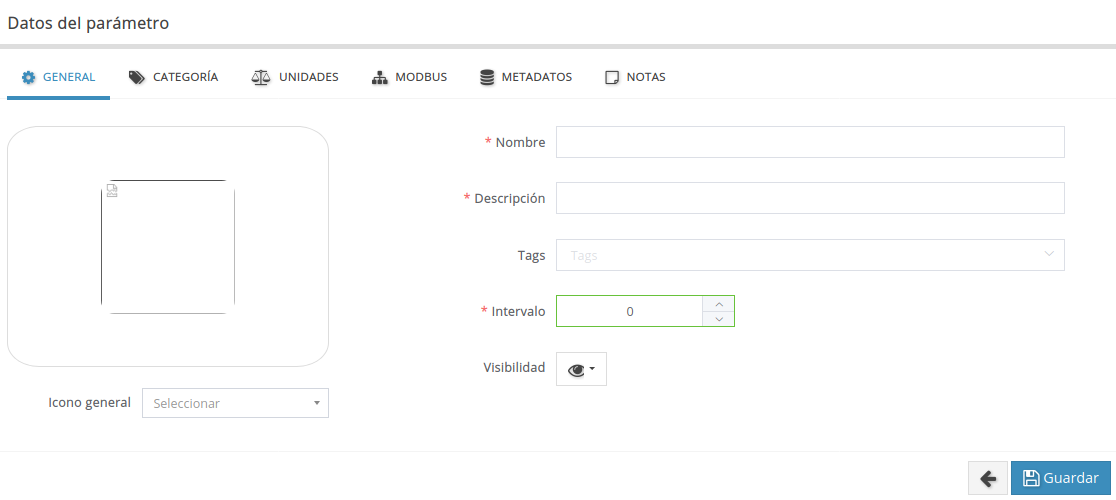
\includegraphics[width=\textwidth, keepaspectratio]{img/lib0}
  \caption{Añadir parámetro a librería kiconex - Pestaña general}
  \label{figura:lib0}
\end{figure}

\begin{figure}[H]
  \centering
  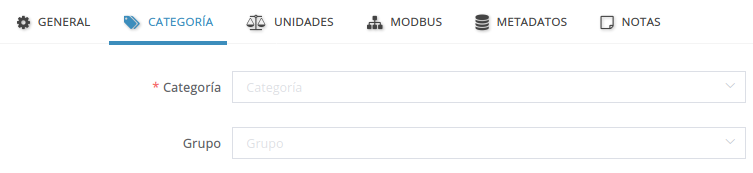
\includegraphics[width=\textwidth, keepaspectratio]{img/lib1}
  \caption{Añadir parámetro a librería kiconex - Pestaña categoría}
  \label{figura:lib1}
\end{figure}

\begin{figure}[H]
  \centering
  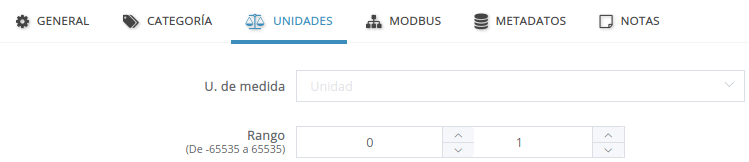
\includegraphics[width=\textwidth, keepaspectratio]{img/lib2}
  \caption{Añadir parámetro a librería kiconex - Pestaña unidades}
  \label{figura:lib2}
\end{figure}

\begin{figure}[H]
  \centering
  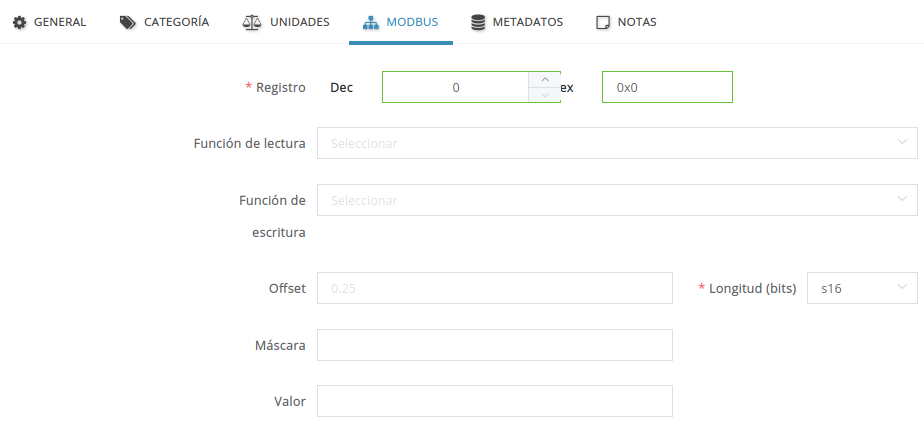
\includegraphics[width=\textwidth, keepaspectratio]{img/lib3}
  \caption{Añadir parámetro a librería kiconex - Pestaña modbus}
  \label{figura:lib3}
\end{figure}

\begin{figure}[H]
  \centering
  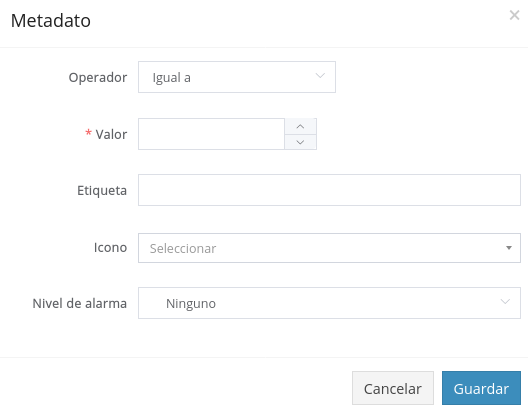
\includegraphics[width=12cm, keepaspectratio]{img/lib4}
  \caption{Añadir parámetro a librería kiconex - adición de metadato}
  \label{figura:lib4}
\end{figure}

\section{Programación dispositivo wireless}
\label{sec:programacionesp32}
Llegados a este punto, hay que buscar la forma de conectar de forma inalámbrica los muebles de refrigeración: murales de lácteos, vitrinas expositoras, semimurales e islas de congelados. Para ello se ha diseñado un nuevo dispositivo que se conecta de forma cableada al control del equipo deseado e intercambia información con la plataforma IoT a través de una red WiFi. Ya se describió en el \hyperref[chap:estadoArte]{capítulo anterior} el hardware a emplear, el ESP32-PoE de Olimex, y se explicó el funcionamiento de una red kiconex. Es por ello que el software del ESP32 debe tener una serie de requisitos:

\begin{itemize}
  \item Comunicación: debe disponer de una interfaz de configuración de red, tanto de la red Modbus como de la red TCP/IP.
  \item Esclavo Modbus TCP: debe ser capaz de recibir las tramas Modbus TCP del maestro kibox, entenderlas y procesarlas para extraer cada campo.
  \item Maestro Modbus RTU: a través de la información extraída de la trama TCP recibida, enviar una nueva trama a través de Modbus RTU.
  \item Respuesta: es necesario repetir el proceso a la inversa: recibir la respuesta a la trama enviada por Modbus RTU, extraer la información y reenviarla como respuesta a la trama Modbus TCP recibida previamente desde el Maestro kibox.
\end{itemize}

\subsection{Librería para la interfaz de configuración}
\label{subsec:interfazKiwi}
Para la interfaz se parte de la librería WiFiManager de Khoi Hoang~\cite{libreriaWiFigithub} \href{https://github.com/khoih-prog/ESP_WiFiManager}{(consultar su enlace en la bibliografía para más información)}. Dicha librería ha sido modificada por completo para adaptarla a las necesidades de diseño del kiwi:

\begin{enumerate}
  \item Interfaz en cualquier modo: accesible tanto en modo AP (para realizar la configuración), como en modo cliente WiFi (para ver y cambiar la configuración realizada).
  \item Medio de conexión: permite seleccionar Ethernet o WiFi.
  \item Diseño: logo de kiwi y colores de kiconex.
  \item Nuevas ventanas con más opciones, como se muestra en la \hyperref[figura:ventanasKiwi]{Figura~\ref{figura:ventanasKiwi}}:

  \begin{figure}[H]
    \centering
    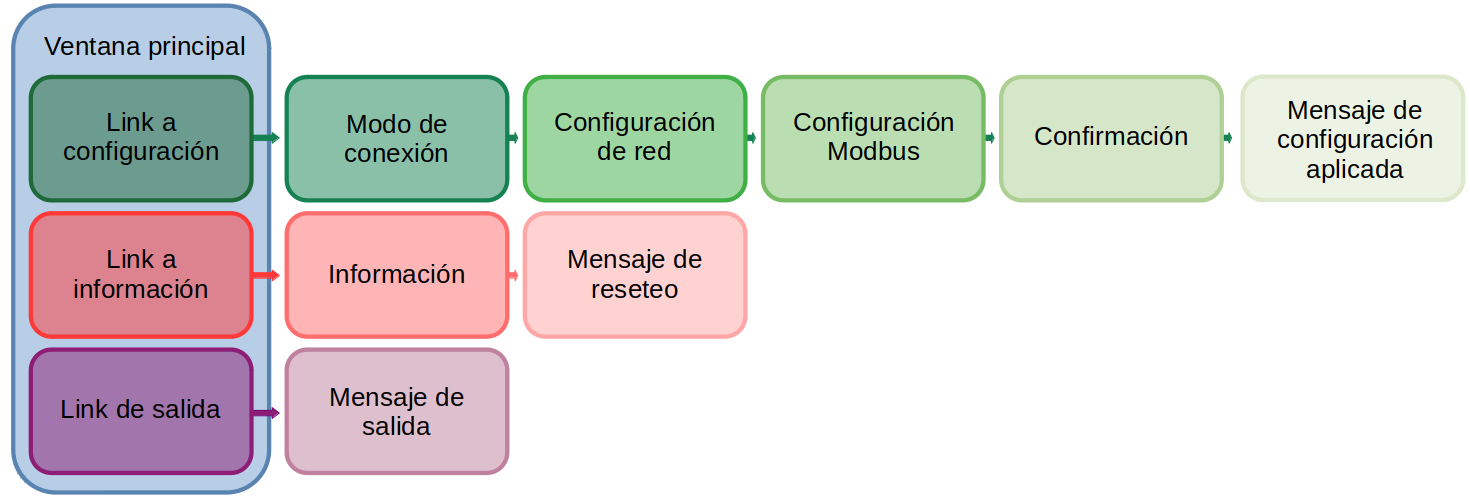
\includegraphics[width=\textwidth, keepaspectratio]{img/ventanasKiwi}
    \caption{Ventanas interfaz kiwi}
    \label{figura:ventanasKiwi}
  \end{figure}
\end{enumerate}

La nueva librería resultado de aplicar los anteriores cambios se ha bautizado con el nombre de KiWiManager. Su uso dentro del código principal es el siguiente:

\begin{itemize}
  \item Configuración inicial:

\begin{lstlisting}
#include "./KiWiManager/src/KiWiManager.h"
#include "./KiWiManager/src/KiWiManager.cpp"

#define USE_AVAILABLE_PAGES     false
#define SHOW_AP_DEBUG           true
#define CONFIGURATION_TIMEOUT   90      //time in seconds  

// For some unknown reason webserver can only be started once per boot up
// so webserver can not be used again in the sketch.
#define WIFI_CONNECT_TIMEOUT        60000L
#define WHILE_LOOP_DELAY            5000L
#define WHILE_LOOP_STEPS            (WIFI_CONNECT_TIMEOUT / ( 3 * WHILE_LOOP_DELAY ))

// SSID and PW for Config Portal
const char* HOSTNAME = "kiwigw";
String ssid = "KiWi_" + String(ESP_getChipId(), HEX);
const char* password = "*********";
byte mac[6];

// SSID and PW for your Router
String Router_SSID;
String Router_Pass;

KiWiManager KiWiPortal(HOSTNAME);

void setup()
{
  KiWiPortal.begin();
}
\end{lstlisting}

\item Acceso al modo AP:

\begin{lstlisting}
  KiWiPortal.setDebugOutput(SHOW_AP_DEBUG);
  KiWiPortal.showAvailablePages(USE_AVAILABLE_PAGES);
  KiWiPortal.setMinimumSignalQuality(15);

  Router_SSID = KiWiPortal.getSSID();
  Router_Pass = KiWiPortal.WiFi_Pass();

  if (Router_SSID != "")
  {
    KiWiPortal.setConfigPortalTimeout(CONFIGURATION_TIMEOUT); //If no access point name has been previously entered disable timeout.
    #ifdef MBMainDebug
      Serial.println("Stored: SSID = " + Router_SSID + ", Pass = " + Router_Pass);
      Serial.print("Timeout ");
      Serial.print(CONFIGURATION_TIMEOUT);
      Serial.println("s");
    #endif
  }
  else{
    #ifdef MBMainDebug
      Serial.println("No timeout");
    #endif
  }

  if (!KiWiPortal.startConfigPortal((const char *) ssid.c_str()/*, password*/)){
    #ifdef MBMainDebug
      Serial.println("Not connected to WiFi but continuing anyway.");
    #endif
  }else{
    #ifdef MBMainDebug 
      Serial.println("WiFi connected in WiFiManager.");
    #endif
  }
\end{lstlisting}
  
  \item Conexión en modo cliente WiFi:
  
\begin{lstlisting}
  KiWiPortal.setDebugOutput(SHOW_AP_DEBUG);
  KiWiPortal.showAvailablePages(USE_AVAILABLE_PAGES);
  KiWiPortal.setMinimumSignalQuality(40);

  Router_SSID = KiWiPortal.getSSID();
  Router_Pass = KiWiPortal.getPASS();
  IPAddress ip = KiWiPortal.getIP();
  IPAddress gw = KiWiPortal.getGW();
  IPAddress sn = KiWiPortal.getSN();
  IPAddress dns1 = KiWiPortal.getDNS1();
  IPAddress dns2 = KiWiPortal.getDNS2();

  WiFi.mode(WIFI_STA);
  WiFi.config(ip,gw,sn,dns1,dns2);
  WiFi.begin(Router_SSID.c_str(),Router_Pass.c_str());
  
  while ( (WiFi.status() != WL_CONNECTED) && (millis() - startedAt < WIFI_CONNECT_TIMEOUT ) )
  {
      #ifdef MBMainDebug
        Serial.print(".");
      #endif 
      int i = 0;
      while ((!WiFi.status() || WiFi.status() >= WL_DISCONNECTED) && i++ < WHILE_LOOP_STEPS)
      {
        delay(WHILE_LOOP_DELAY);
      }
  }
\end{lstlisting}
    
    \item Conexión en modo cliente Ethernet:
  
\begin{lstlisting}
  KiWiPortal.setDebugOutput(SHOW_AP_DEBUG);
  KiWiPortal.showAvailablePages(USE_AVAILABLE_PAGES);
  KiWiPortal.setMinimumSignalQuality(15);

  configState = KiWiPortal.startEthernetClientConfigPortal((const char *) ssid.c_str());
\end{lstlisting}  

\end{itemize}

\subsection{Librería para maestro Modbus RTU}
\label{subsec:maestroRTUkiwi}

Para esto se ha empleado la librería Modbus RTU del usuario smarmengol (Samuel Marco) en github. Para usarla dentro del código y poder enviar mensajes Modbus y recibir las respuestas, se emplea el siguiente código:

\begin{itemize}
  \item Inicialización:
  
  \begin{lstlisting}
    #include "../KiWiModbusRTU/KiWiModbusRtu.h"
    #include "../KiWiModbusRTU/KiWiModbusRtu.cpp"
    
    Modbus master(u8id, u8serno, u8txenpin);
    
    master->begin(u32speed);      // baud-rate
    master->setTimeOut(timeOut);  // Tiempo entre reintentos
  \end{lstlisting}  

  \item Uso:
  
  \begin{lstlisting}
  uint8_t rtuCommunication = 1;
  uint8_t ret = 0;

  modbus_t telegrama[2];
  uint8_t w_id = READ_index;

  if (rw1 == 1) w_id = WRITE_index;

  this->_u8state = 0;

  /**
  Struct with Modbus RTU parameters
  telegrama[0].u8id       slave ID
  telegrama[0].u8fct      Modbus Function Code
  telegrama[0].u16RegAdd  Start address
  telegrama[0].u16CoilsNo Number of registers or coils to read/write
  telegrama[0].au16reg    Pointer to memory array
  */
  telegrama[rw1].u8id = au16data[ID_index];         // slave ID
  telegrama[rw1].u8fct = au16data[FN_index];        // function code
  telegrama[rw1].u16RegAdd = au16data[START_index]; // star address
  telegrama[rw1].u16CoilsNo = au16data[LONG_index]; // number of registers/coils
  telegrama[rw1].au16reg = au16data + w_id;         // pointer to memory array

  while (rtuCommunication)
  {
    switch (this->_u8state)
    {
      case 0:
        this->_u8state++;
        break;
      case 1:
        master->query(telegrama[rw1]); // send query (only once)
        this->_u8state++;
        break;
      case 2:
        ret = master->poll(); // check message reception
        /**
           When generating the request to the slave, the master is in
           COM_IDLE mode, and after that its status would be COM_WAITING
                 COM_IDLE=0 ; COM_WAITING=1
        */
        if (master->getState() == COM_IDLE)
        {
          rtuCommunication = 0;
        }
        break;
    }
  }
  \end{lstlisting} 
\end{itemize}

\subsection{Librería para esclavo Modbus TCP}
\label{subsec:esclavoTCPkiwi}

En este caso se ha diseñado por completo una librería cuya función es esperar la recepción de mensajes transmitidos por TCP/IP y con destino a la IP concreta del dispositivo. Estos mensajes son procesados y enviados vía Modbus RTU empleando la librería \textit{Modbus RTU} del apartado anterior. Es decir se trata de una librería puente, por lo que se ha bautizado con el nombre de KiWiModbusBridge. Su uso dentro del código principal es el siguiente:

\vspace*{\fill}

\begin{lstlisting}
// Modbus bridge library
#include "./KiWiModbusBridge/KiWiModbusBridge.h"
#include "./KiWiModbusBridge/KiWiModbusBridge.cpp"

/**
 *  ModBus RTU Configuration
 *  u8id : id = 0 for master, = 1..247 for slaves
 *  u8serno : serial port (0 for Serial)
 *  u8txenpin : 0 for RS-232 and USB-FTDI 
 *               any value > 1 para RS-485
 */
uint8_t u8id = 0; 
uint8_t u8serno = 0;   
uint8_t u8txenpin = 5;  

KiWiModbusBridge slave(u8id, u8txenpin, u8txenpin);

long rtu_br;
unsigned int tcp_port;

void setup()
{
  rtu_br=9600;
  tcp_port=502;
  slave.begin(tcp_port, rtu_br);
}

void loop()
{
  slave.run();
}

\end{lstlisting}

\vspace*{\fill}

\clearpage

En la \hyperref[figura:flujoLibreriaPuente]{Figura~\ref{figura:flujoLibreriaPuente}} se describe la lógica de funcionamiento de esta librería:

\begin{figure}[H]
  \centering
  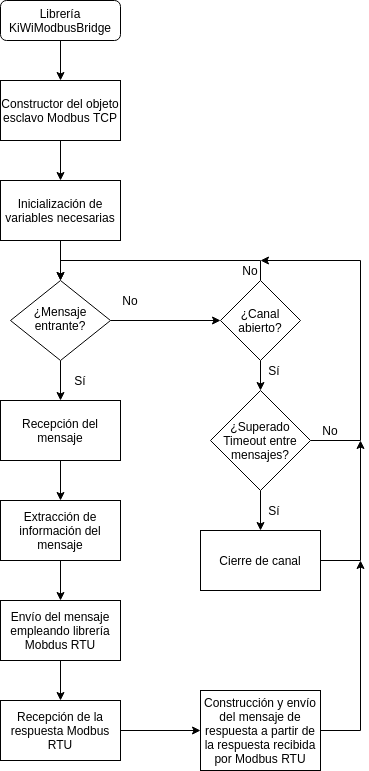
\includegraphics[width=10cm, keepaspectratio]{img/flujoLibreriaPuente}
  \caption{Flujo de programa pasarela TCP-RTUxxx}
  \label{figura:flujoLibreriaPuente}
\end{figure}

\subsection{Código principal}
\label{subsec:mainCodeKiwi}

El código principal del software de kiwi se encarga de integrar cada una de las librerías anteriores y de gestionar el flujo de programa. Su lógica de funcionamiento se recoge en el siguiente diagrama:

\begin{figure}[H]
  \centering
  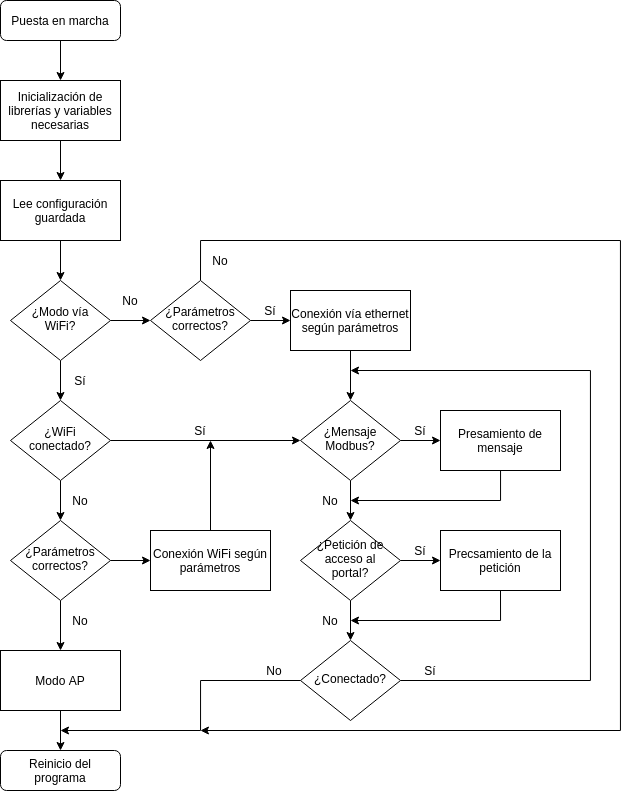
\includegraphics[width=15cm, keepaspectratio]{img/flujoProgramaPrincipal}
  \caption{Flujo de programa del código principal de kiwi}
  \label{figura:flujoProgramaPrincipal}
\end{figure}


\subsection{Integración de todos los elementos del sistema}
\label{subsec:integracionComponentes}

Ya esta todo listo para conectarlo a la red kiconex. Como ya se ha mencionado, los equipos del supermercado se comunican con la plataforma a través del kibox y del kiwi. Por ello, lo primero es crear la instalación del supermecado en la plataforma IoT, utilizando el id único de cada kibox, y después se añaden a dicha instalación cada uno de los equipos: 

\begin{itemize}
  \item Las centrales, las cámaras de refrigeración y los equipos de clima, se conectan de forma cableada al kibox a través de Modbus RTU, por lo que en la plataforma se añaden indicando su librería de registros y el puerto y la dirección Modbus.
  \item En el caso de los muebles de refrigeración, se conectan de forma cableada con el kiwi a través de Modbus RTU. Dado que la comunicación se realiza a través del mismo kiwi, vía TCP, cada mueble se añade a la instalación indicando la librería de registros del control, la IP del kiwi, y la dirección Modbus del control. 
\end{itemize}

La \hyperref[figura:esquemaConexion]{Figura~\ref{figura:esquemaConexion}} siguiente, indica el esquema de conexión física de cada equipo.

\begin{figure}[H]
  \centering
  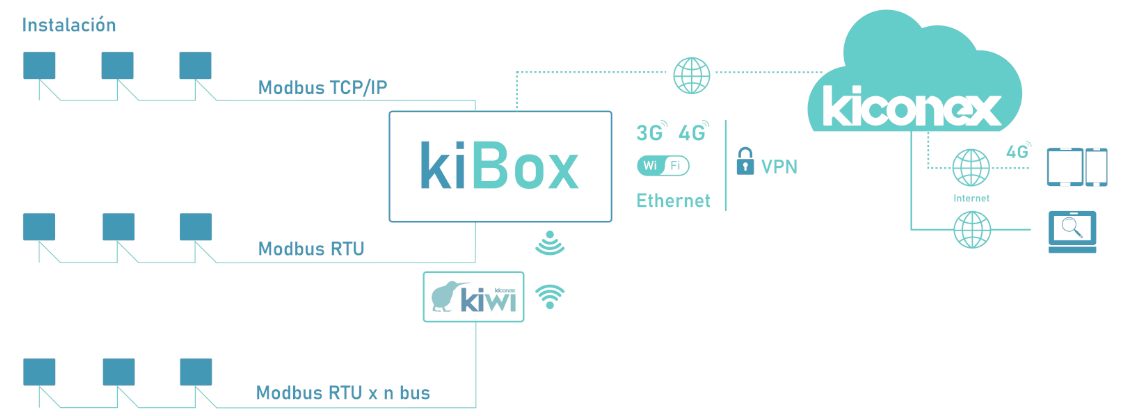
\includegraphics[width=\textwidth, keepaspectratio]{img/esquemaConexion}
  \caption{Esquema conexión equipos supermercado}
  \label{figura:esquemaConexion}
\end{figure}

La \hyperref[figura:creacionInstalacion1]{Figura~\ref{figura:creacionInstalacion1}} y la \hyperref[figura:creacionInstalacion2]{Figura~\ref{figura:creacionInstalacion2}} muestran el proceso de creación de una instalación en la plataforma IoT de kiconex y la \hyperref[figura:adicionDispositivo1]{Figura~\ref{figura:adicionDispositivo1}} y la \hyperref[figura:adicionDispositivo2]{Figura~\ref{figura:adicionDispositivo2}} el proceso de adición de dispositivos a la misma. Se observa como cada instalación necesita ese \textit{UUID} único y específico del kibox al que se enlaza, además de una configuración de los posibles puertos de los que disponga dicho modelo de kibox. Por otro lado, el dispositivo necesita que se especifique su configuración Modbus: TCP o RTU, IP, dirección, puerto, etc. Finalmente, la instalación tiene el aspecto de la \hyperref[figura:instalcionCreada]{Figura~\ref{figura:instalcionCreada}}.



\vspace*{\fill}

\begin{figure}[H]
  \centering
  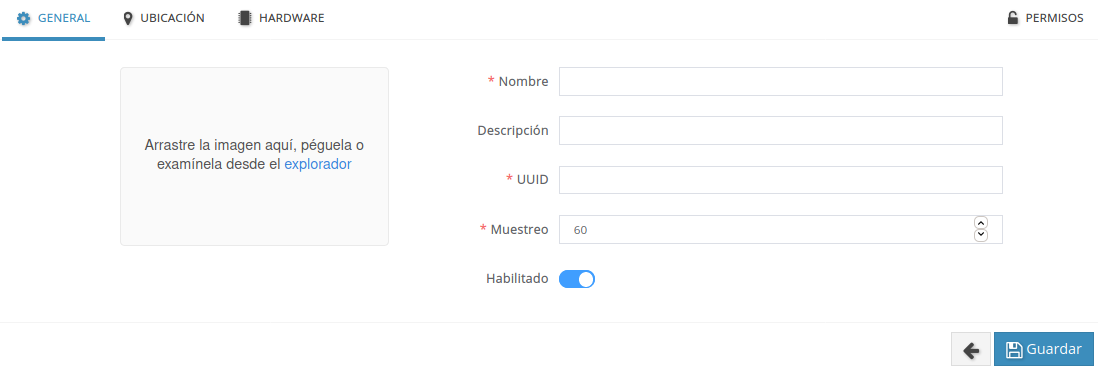
\includegraphics[width=\textwidth, keepaspectratio]{img/creacionInstalacionGeneral}
  \caption{Creación instalación en plataforma IoT - Datos generales}
  \label{figura:creacionInstalacion1}
\end{figure}

\vspace*{\fill}

\begin{figure}[H]
  \centering
  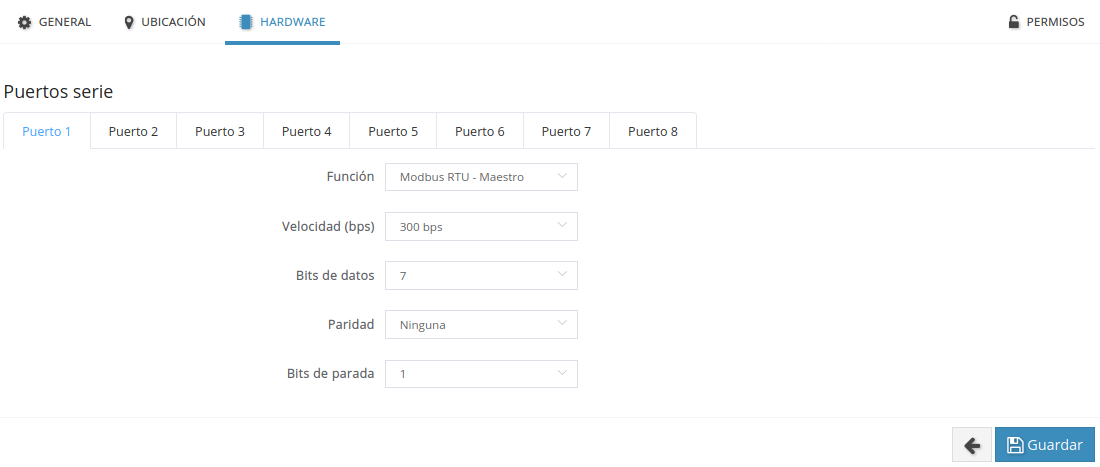
\includegraphics[width=\textwidth, keepaspectratio]{img/creacionInstalacionHardware}
  \caption{Creación instalación en plataforma IoT - Hardware kibox}
  \label{figura:creacionInstalacion2}
\end{figure}

\vspace*{\fill}

\begin{figure}[H]
  \centering
  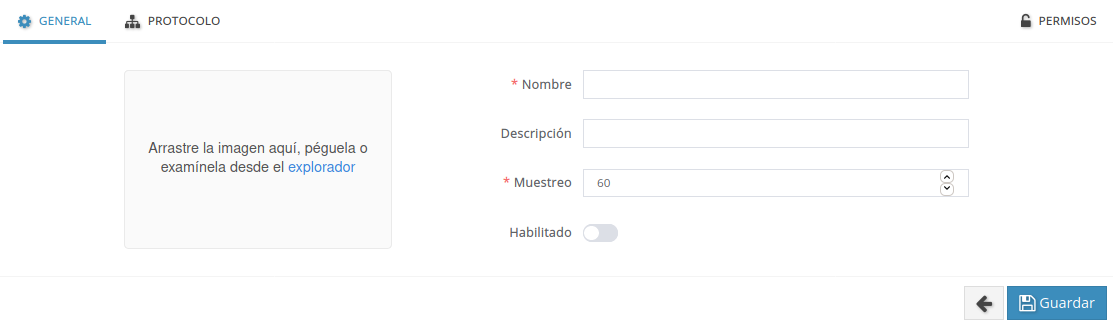
\includegraphics[width=\textwidth, keepaspectratio]{img/creacionDispositivoGeneral}
  \caption{Adición de dispositivo a la instalación - Datos generales}
  \label{figura:adicionDispositivo1}
\end{figure}

\vspace*{\fill}

\begin{figure}[H]
  \centering
  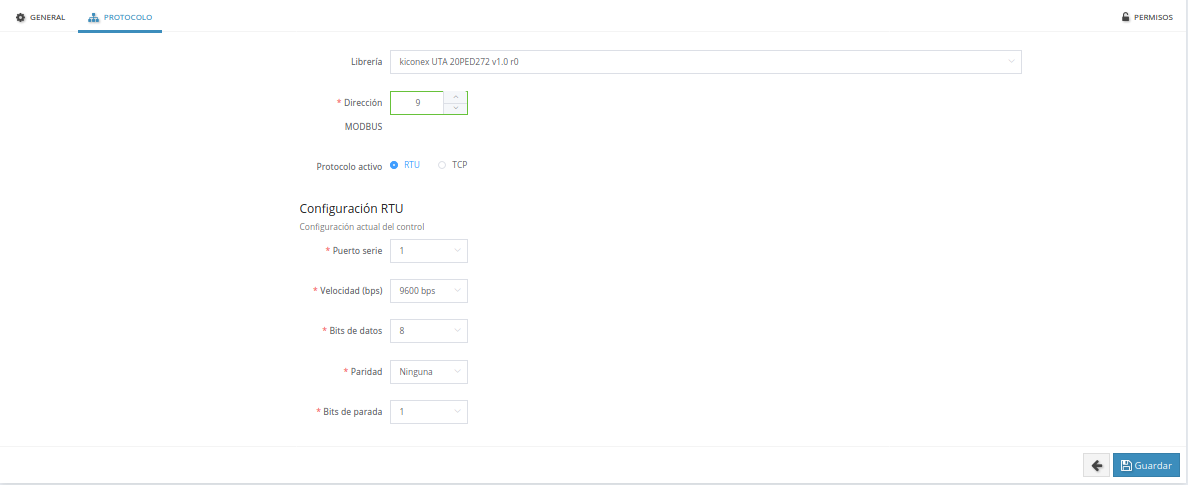
\includegraphics[width=\textwidth, keepaspectratio]{img/creacionDispositivoProtocolo}
  \caption{Adición de dispositivo a la instalación - Datos Modbus dispositivo}
  \label{figura:adicionDispositivo2}
\end{figure}

\vspace*{\fill}

\begin{figure}[H]
  \centering
  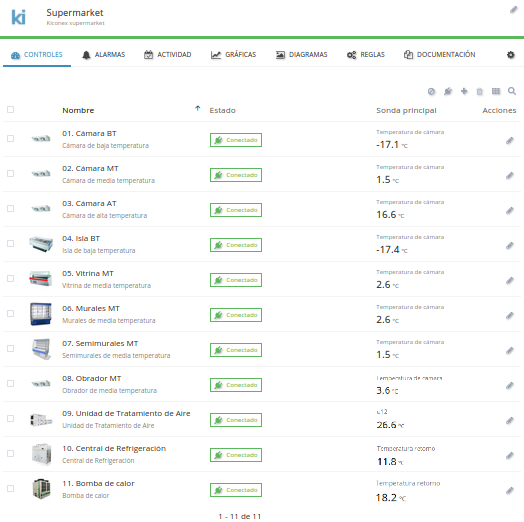
\includegraphics[width=\textwidth, keepaspectratio]{img/instalacionConectada}
  \caption{Instalación supermercado creada}
  \label{figura:instalcionCreada}
\end{figure}

\vspace*{\fill}